\pdfminorversion=4
\documentclass[aspectratio=169]{beamer}
\mode<presentation>
{
  \usetheme{default}
  \usecolortheme{default}
  \usefonttheme{default}
  \setbeamertemplate{navigation symbols}{}
  \setbeamertemplate{caption}[numbered]
  \setbeamertemplate{footline}[frame number]  % or "page number"
  \setbeamercolor{frametitle}{fg=white}
  \setbeamercolor{footline}{fg=black}
} 
\usetheme{Madrid}
\usepackage{lmodern}
\usepackage{hyperref}
\usepackage{apacite}
\usepackage[utf8]{inputenc}
\usepackage[spanish]{babel}

\usepackage{xcolor}
\xdefinecolor{dianablue}{rgb}{0.18,0.24,0.31}
\xdefinecolor{darkblue}{rgb}{0.1,0.1,0.7}
\xdefinecolor{darkgreen}{rgb}{0,0.5,0}
\xdefinecolor{darkgrey}{rgb}{0.35,0.35,0.35}
\xdefinecolor{darkorange}{rgb}{0.8,0.5,0}
\xdefinecolor{darkred}{rgb}{0.7,0,0}
\definecolor{darkgreen}{rgb}{0,0.6,0}
\definecolor{mauve}{rgb}{0.58,0,0.82}
% \setbeamertemplate{background}{\tikz[overlay,remember picture]\node[opacity=0.1]at (current page.center){\includegraphics[width=13cm]{Psicoven.png}};}
\usepackage{tikz}
\usepackage{kantlipsum}

\setbeamercolor{normal text}{fg=black}

\begin{document}
\colorlet{beamer@blendedblue}{dianablue}


\setbeamercolor*{palette primary}{fg=white,bg=dianablue}
\setbeamercolor*{palette secondary}{fg=white,bg=dianablue}
\setbeamercolor*{palette tertiary}{fg=white,bg=dianablue}

\setbeamercolor{frametitle}{fg=white, bg=dianablue}
\setbeamercolor*{title}{fg=white, bg=dianablue}

\setbeamercolor{section in toc}{fg=black, bg=dianablue}

\author[Juan C. Correa, Ph.D.]{Juan C. Correa, Ph.D.}


\title[Python: Pandas]{Aprendiendo Python para Análisis Estadísticos}
\subtitle{Pandas}
	%\subtitle{}
\institute[]{
	\color{blue}\Email  \href{mailto:j.correa.n@gmail.com}{j.correa.n@gmail.com}
}
\pgfdeclareimage[height=0.7cm]{python}{python}
\logo{\pgfuseimage{python}}
\setbeamertemplate{caption}[numbered]
\date[Junio 2021]{\textcolor{blue}{\url{https://correajc.com/}}}

%\subject{}
\setbeamercolor{background canvas}{bg=white}
%\setbeamertemplate{navigation symbols}{}

\begin{frame}
	\titlepage
\end{frame}

\begin{frame}
\begin{block}{Objetivo de esta Charla}
\vspace{0.3cm}
\begin{itemize}
    \item Comprender los alcances conceptuales y operativos de la librería Pandas como herramienta útil para el análisis estadístico de datos.
    \item Introducir, a través de un tutorial, los elementos más básicos de la librería de Pandas
\end{itemize}

\end{block}
\end{frame}

\begin{frame}{~~~~~~~~~~~~~~~~~~~~~~~~~~~~~~~~~~~~~~~~~~~~~~~~~~~~~~~~~~~~~~~~~~~~~~~~~~~~~~~~~Agenda}
\tableofcontents
\end{frame}


\section{Pandas: Breve Descripción}
\begin{frame}
\centering
\begin{figure}
\centering

\includegraphics[width=.6\textwidth]{pandas.jpg}
\end{figure}
\Huge
Breve Descrpipción
\end{frame}

\begin{frame}
Pandas proporciona una variedad de funciones diseñadas para trabajar con datos estructurados de una manera rápida, fácil y expresiva \cite{McKinney2012}. \\
\vspace{0.4cm}
Es uno de los ingredientes críticos que permiten que Python sea un entorno de análisis de datos potente y productivo.\\
\vspace{0.4cm}
Los datos estructurados que se manejan con Pandas se implementan a través de sus dos caballos de fuerza más importantes: \textbf{\textit{Series}} y \textbf{\textit{Dataframes}}.
\end{frame}

\subsection{Series}
\begin{frame}
En Python, un objeto \textbf{\textit{Series}} es un vector unidimensional que contiene un conjunto de datos (de cualquier clase \texttt{NumPy}) junto a su conjunto de etiquetas de datos (las etiquetas van por fila).
\begin{figure}
\centering
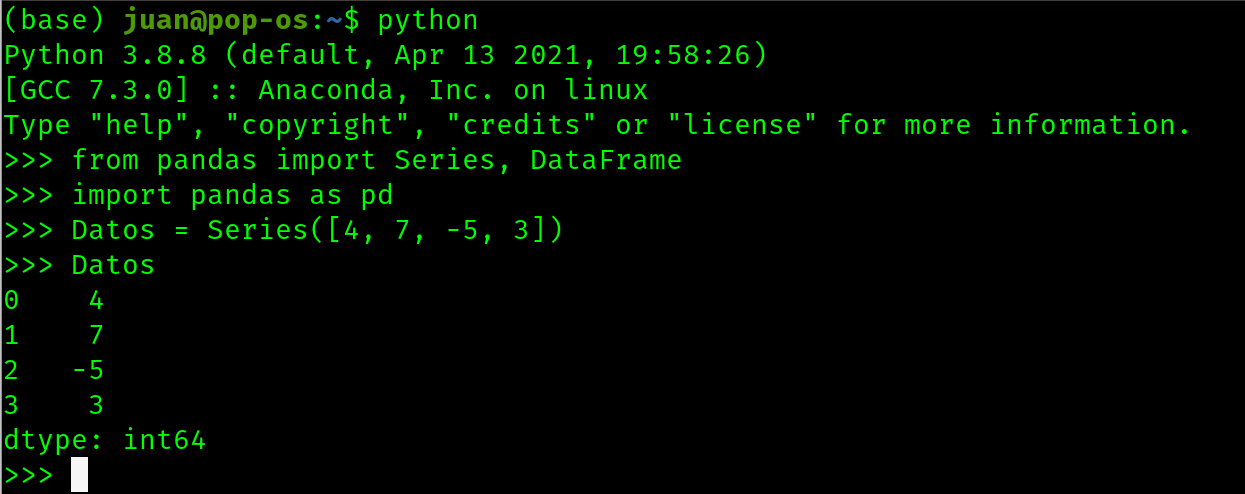
\includegraphics[width=.8\textwidth]{p1.png}
\end{figure}
\end{frame}

\begin{frame}
El objeto \texttt{Datos} tiene cuatro valores (4, 7, -5, 3) cada uno de los cuales tiene su propia etiqueta (0, 1, 2, 3).
\begin{figure}
\centering
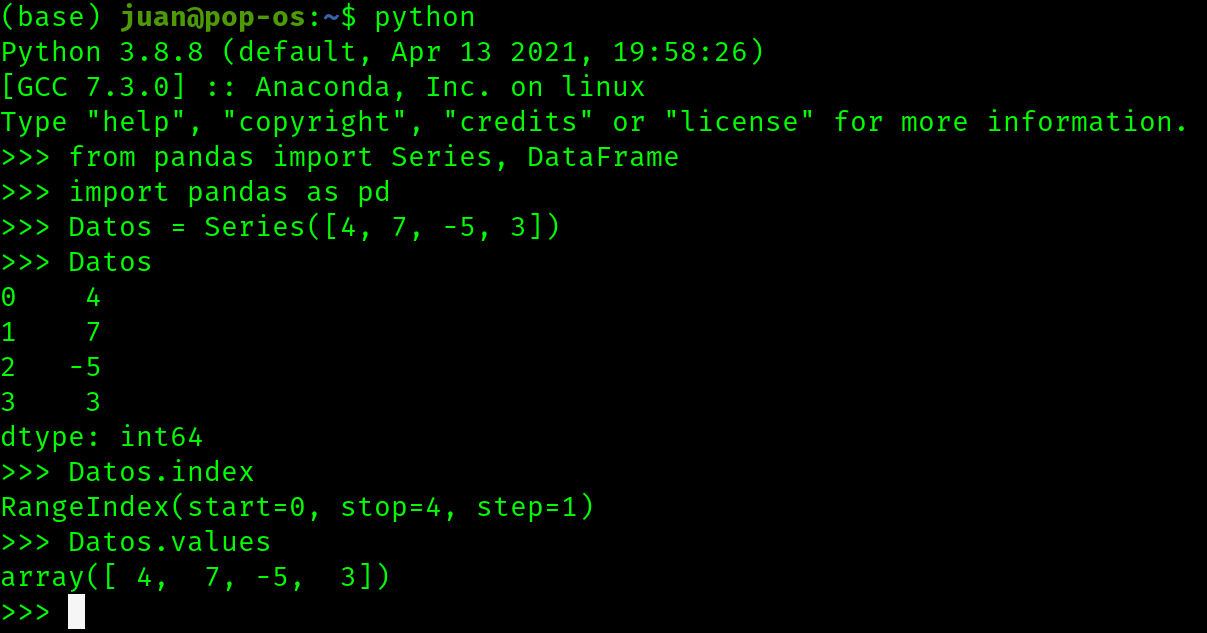
\includegraphics[width=.8\textwidth]{p2.png}
\end{figure}
\end{frame}


\begin{frame}
Vamos a crear el objeto \texttt{Datos2} a partir de otro tipo de estructura de datos conocida como dict y que aquí llamamos \texttt{sdata}.
\begin{figure}
\centering
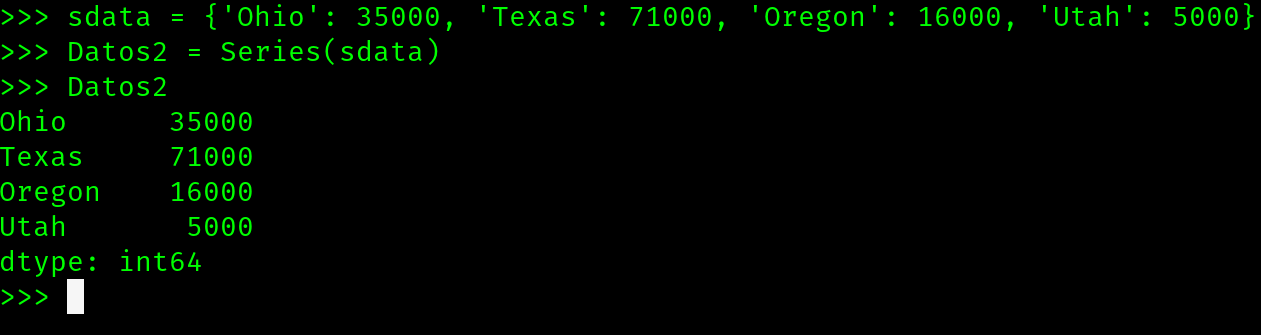
\includegraphics[width=.8\textwidth]{p3.png}
\end{figure}
Entre las páginas 112 a 115 del libro de texto de \citeauthor{McKinney2012} \citeyear{McKinney2012} se presentan otras características de los objetos \texttt{Series}.
\end{frame}

\subsection{Dataframes}
\begin{frame}
Los objetos de tipo \texttt{Dataframes} son objetos tipo hoja de cálculo (filas por columnas) con etiquetas para filas y columnas.   
\begin{figure}
\centering
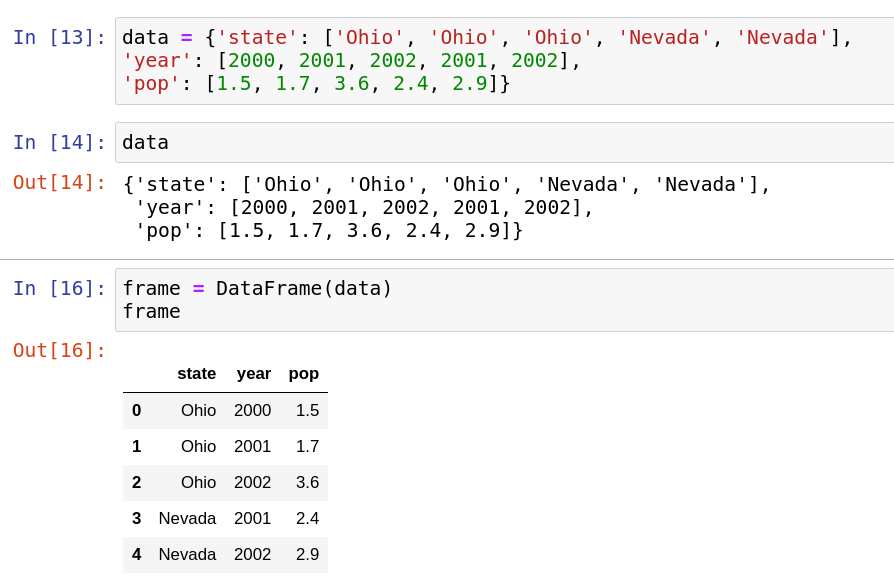
\includegraphics[width=.7\textwidth]{p4.png}
\end{figure}
\end{frame}



\begin{frame}[allowframebreaks]{Referencias}
\tiny
\bibliographystyle{apacite}
\bibliography{refs} 
\end{frame}


\end{document}